In diesem Kapitel wird der Quicktest in \ac{tpt} überführt.
Es werden die Einstellungen in \ac{tpt} getroffen. Es werden die Testfälle erstellt und schließlich wird ein Skript 
geschrieben, das die Testfälle automatisiert generiert.
\section*{C Platform Konfiguration}
\begin{description}
\item[Compiler auswählen] Pfad zu mingw Installation (C Compiler)% /scwcc\_tools/FRD/tools/pc/mingw %installiert zu einem installierten Compiler
\item[Sourcen auswählen] nach design pattern alle <Komponente>\_Task.c %und Einbinden der Datafield C Dateien im Wrapper%Dateien Diese werden später gelinkt und kompiliert, zu analysierende Sourcen müssen auf analysieren gestellt werden
% dabei werden die ausgewählten Sourcen kompiliert und diejenigen, die auf zu analysieren gestellt sind, werden analysiert
% für GSIL: alle \_Task.c auf set analyze setzen
\item[Scheduler] Funktionsaufrufe in Task Dateien
\item[Step size] 125\textmu s
\end{description}
Vom bestehenden Quicktest gibt es einen Ordner,
%(scwcc\_ec\_tc/Integrationstest/Softcar/SIL\_Files/QTestFunctions)
wo pro Komponente die Funktionen, in denen die Schnittstellen definiert sind, aufgeführt sind (siehe Kapitel 3).
%Des Weiteren wird im Wrapper die Datei eingebunden, die die Datafield C Dateien einbindet, in denen die Signale definiert sind.

\section*{Testfallerstellung}
%Die Daten der Schnittstellen können aus der Datafield wie in der Analyse des bestehenden Quicktests entnommen werden.
Die notwendigen Schnittstelleninformation für die Testfallerstellung können aus der Datafield entnommen werden (siehe Kapitel 3).
%Die notwendigen Daten für die Testfallerstellung werden wie in der Analyse des Softcar-Quicktests unter Generieren derQuicktest.c entnommen.
Das physikalische Limit wird nicht vom bestehenden Softcar-Quicktest aufgenommen, da es wie vorher beschrieben ein Relikt ist und nicht mehr benötigt wird.
In \ac{tpt} werden die Testfälle als Step Liste mit folgendem Inhalt erstellt:
\begin{description}
\item[Channel Step] Ausgangssignal auf einen der Werte zuweisen
\item[Compare Step] Eingangssignal mit Wert vergleichen, falls float: mit 0,00001 Fehlertoleranz
\item[wait] @
\end{description}
%Für alle Werte werden nacheinander die Testfälle in die Step Liste geschrieben.
Hier ist ein Beispiel eines Testfalls in der Step Liste:
\begin{figure}[h]
\centering
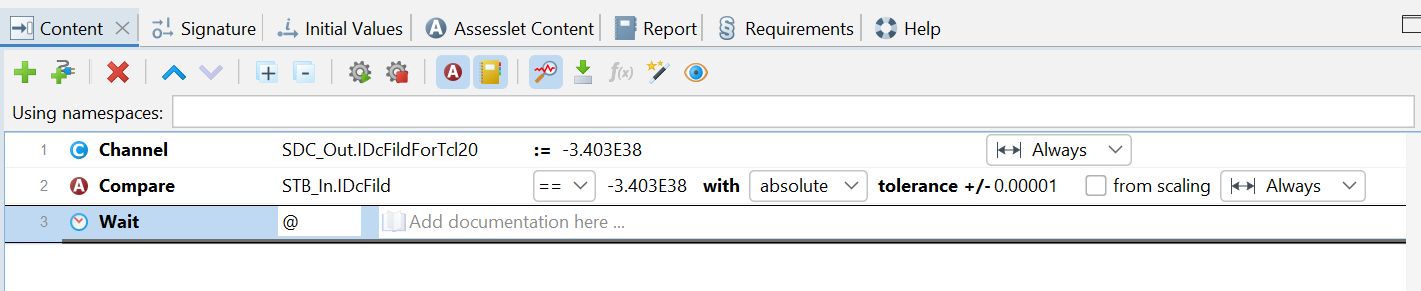
\includegraphics[scale=.6,]{Bilder/Quicktest/Testfallerstellung.png}
\caption{Schnittstellen Testdesign}
\end{figure}